\subsection{Validazione e Collaudo}
Questa fase comincia subito dopo la fase precedente e finisce con la data di consegna per la \textit{Revisione di Accettazione}, ovvero dal 09-04-2020 al 03-05-2020.\\
In questo periodo verranno creati ulteriori test per verificare il corretto funzionamento del prodotto. Se tutte le scadenze imposte dal gruppo vengono rispettate il tempo in eccesso viene occupato per la realizzazione di requisiti opzionali, concordati con il committente. 
\subsubsection{Completamento dell'implementazione e raffinamento delle funzionalità}
\paragraph{Incremento VIII}\textit{}\\
\textit{Dal 09-04-2021 al 16-04-2021}. \\ 
Nel seguente incremento il team s'impegnerà a terminare i lavori avviati nel periodo precedente e ultimare i seguenti obbiettivi:
\begin{itemize}
	\item Viene implementata una gestione della sessione;
	\item Viene implementato un componente per l'esportazione dei parametri di configurazione dell'applicazione;
	\item Viene implementato un componente per l'importazione dei parametri di configurazione dell'applicazione.
\end{itemize}			
\textbf{Attività}			
\begin{itemize}
\item \textbf{Stesura:} incremento della documentazione da allegare al prodotto;
\item \textbf{Verifica dei documenti} 
\item \textbf{Progettazione:} progettazione di un sistema per la gestione della sessione;
\item \textbf{Codifica:} codifica dei componenti per l'importazione e l'esportazione dei parametri di configurazione dell'applicazione;
\item \textbf{Verifica software:} verifica sulle funzionalità software aggiunte.
\end{itemize}
\paragraph{Incremento IX}\textit{}\\
\textit{Dal 16-04-2021 al 23-04-2021}. \\ 
Nel seguente incremento il team s'impegnerà a terminare i lavori avviati nel periodo precedente e ultimare i seguenti obbiettivi:
\begin{itemize}
	\item Viene implementato una sistema di \glo{widget} per l'utilizzo dell'applicazione;
	\item Viene realizzata una guida introduttiva per l'utilizzo dell'applicazione.
\end{itemize}			
\textbf{Attività}			
\begin{itemize}
\item \textbf{Stesura:} incremento della documentazione da allegare al prodotto;
\item \textbf{Verifica dei documenti} 
\item \textbf{Progettazione:} progettazione di un sistema di \glo{widget} e di una guida introduttiva;
\item \textbf{Codifica:} codifica dei componenti per i \glo{widget} e per la guida introduttiva;
\item \textbf{Verifica software:} verifica sulle funzionalità software aggiunte.
\end{itemize}
\subsubsection{Verifica e collaudo}
Il periodo di verifica e collaudo ha inizio il giorno 23-04-2021, alla conclusione degli incrementi, con termine fissato per il giorno 03-05-2021.
\begin{itemize}
	\item \textbf{Incremento e verifica dei documenti:} se fosse necessario, i documenti prodotti dal team verranno integrati;
	\item \textbf{Verifica e collaudo:} vengono creati e applicati un set di test, che hanno lo scopo di portare il prodotto ad un buon livello qualitativo. Il gruppo si focalizzerà sulla sua correttezza e nel rispetto di tutti i requisiti;
	\item \textbf{Codifica:} rilascio dell'ultima versione del prodotto.
\end{itemize}

\begin{landscape}
\begin{figure}[h]
	\centering
	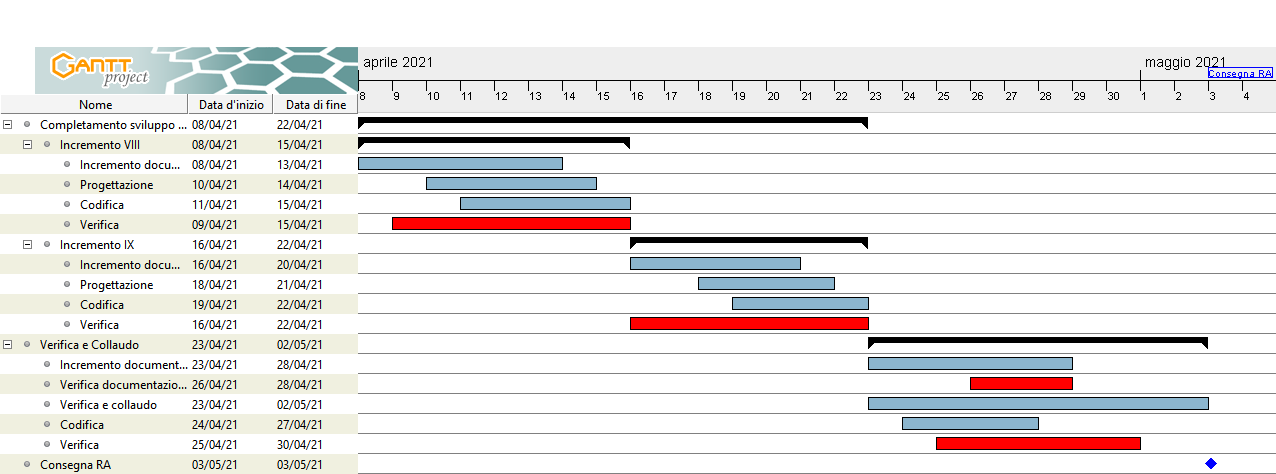
\includegraphics[width=\linewidth]{Images/GanttPianificazioneValidazioneCollaudo.PNG}
	\caption{Diagramma di Gantt dell'attività di Validazione e Collaudo}
\end{figure}
\end{landscape}



